%% TMLR submission — Verifiable Design Conditions for Symbolic Training:
%% two-pole OOD evidence, the decoupling operator, and its ablation
\documentclass{article} % For LaTeX2e
\usepackage{iclr2026_conference,times}
\usepackage{amsmath,amssymb}
\usepackage{booktabs}
\usepackage{graphicx}
\usepackage[hidelinks]{hyperref}
\usepackage{url}

\title{When Does Symbolic Training Generalize Out-of-Distribution?\\
Four Verifiable Design Conditions and an Ablation of the\\
Decoupling Operator}

% 双盲: 不取消注释 \iclrfinalcopy; 作者匿名
\author{Anonymous\\
\small Independent Researcher\\
\small AI assistance: DeepSeek (commercial API language model)}

\begin{document}
\maketitle

\noindent\textbf{AI assistance statement.} This work was developed
in a human--AI collaboration. The research was directed by the
author through an API-hosted model (DeepSeek): the author led the
questions, the experiments, and the judgments; the model was the
interface through which the author's intentions were expressed,
checked, and refined. The model's capabilities have been distilled,
so the author's original knowledge cannot be recovered from any
single interaction; the statements in this paper are the author's
expectation, directed through the model, of recovering as
faithfully as possible the content that distillation has dispersed.
The full collaboration record (session log, phase classification,
artifacts) is available for audit.

\begin{abstract}
A transformer trained on a symbolic task can reach training
accuracy 1.000 while its out-of-distribution (OOD) accuracy
collapses --- or transfers perfectly --- depending on properties of
the \emph{token design} rather than of the task. We reproduce this
two-pole pattern in 45 controlled runs (E12: $32/32$ in the trained
notation versus $0/32$ in an untrained notation of the same
basepoint, and $32/32$ after explicit equivalence statements) and
report per-token OOD curves over epochs for every condition. We
state four verifiable design conditions that organize the pattern:
signal completeness (the decoupling operator $D$ = exclusion +
cancellation + layering), symbol norm, presentation legality, and
intuition precision. The conditions are operational: each has a
two-pole experimental design and a Lean 4 formalization (five
theorems, zero \texttt{sorry}). We ablate the decoupling operator
on 108 fresh runs (10 seeds per condition): layering violations
(one symbol in two roles) prevent OOD recovery entirely
(sequence-level 0/10, per-token $0.92$), missing declarations cap
per-token OOD at $0.238$, and exclusion violations (30\% noise) do
not prevent recovery but slow it significantly (peak epoch $22.7
\to 28.6$, $p = 0.04$). Per-position labels localize the failures:
without declarations only the shared-structure positions recover;
with a dual-role symbol the conflicted role's positions never do.
The pattern and the ablation are stable across model widths
(64/128) and depths (2/4 layers). We report the honest boundary and
what remains open.
\end{abstract}

\section{Introduction}

Transformers trained on algorithmic and symbolic tasks show a
striking asymmetry: high training accuracy, and OOD behavior that
ranges from perfect transfer to complete collapse depending on
seemingly superficial properties of the representation
\citep{power2022grokking, deletang2022chomsky,
lake2018generalization, keysers2020measuring,
hupkes2020compositionality, bahdanau2019systematic,
anil2022exploring, jelassi2023length, raffel2020exploring,
saxton2019analysing, lample2020deep, hendrycks2021measuring,
razeghi2022impact}. A common diagnosis is that the model learns
\emph{representation-bound statistics}: what transfers is what the
training distribution's statistics carry, and nothing else. If that
is the mechanism, then the design of the token system --- the
symbols, their grammar, their presentation --- is not a stylistic
choice but a determinative factor of what the model can
generalize. This paper makes that claim operational.

We study a five-layer token system (basepostulate, concept, symbol,
grammar, presentation) with controlled transformer training on
successor-notation arithmetic, and report three things.

\textbf{(1) A reproduced two-pole pattern.} In 45 runs (3 seeds
$\times$ 3 executions $\times$ 5 conditions, dimension 64, two
layers, 60 epochs), training accuracy reaches 1.000 in every run,
while OOD accuracy is $32/32$ for length extrapolation in the
trained notation, $0/32$ for the same structure in an untrained
notation of the same basepoint, and $32/32$ after explicit
equivalence statements. Two further contrasts sharpen the picture:
position-value bare symbols collapse ($0/30$) while fully expanded
successor chains are stable ($30/30$); and difference problems
(distinguishing $2 \times 2$ from $2 + 2$) transfer when explicitly
declared ($56/56$) but fail without the declaration ($14/28$, truth
bias).

\textbf{(2) Four verifiable design conditions.} We state four
conditions that organize the pattern --- signal completeness,
symbol norm, presentation legality, intuition precision --- each
with a two-pole experimental design and a Lean 4 formalization
(five theorems, zero \texttt{sorry}). The completeness condition is
the decoupling operator $D$ (exclusion + cancellation + layering):
a signal is complete when every declaration it needs is present,
unblurred, unbiased, and unconflated.

\textbf{(3) An ablation of the decoupling operator.} On 39 fresh
runs we violate each clause of $D$ separately and measure per-token
OOD over epochs, with a peak-epoch label (the epoch at which
per-token OOD first reaches 1.0; if it never does, the epoch of
maximal OOD). Layering violations prevent recovery entirely;
missing declarations cap per-token OOD at $0.238$; exclusion
violations slow recovery monotonically; a one-sided-equivalence
manipulation had no effect (a null result we report honestly). The
pattern is stable across widths 64/128 and depths 2/4.

\section{Setup and metrics}

\textbf{Token system.} The five-layer token system is described in
detail in the appendix; the layer separation is the framework's
first hypothesis: basepostulate (axiom base), concept (what things
are), symbol (how things are written), grammar (how symbols are
arranged), presentation (concrete notation: precedence,
associativity). A token is one object; the layers are projections
of it.

\textbf{Training.} Transformer \citep{vaswani2017attention}, dimension
64, two layers, 60 epochs, Adam ($\mathrm{lr}=10^{-3}$), position
cross-entropy on sequence reconstruction, on 250 successor-notation
arithmetic samples (addition and multiplication facts with positive
and negative cases). OOD probes: length extrapolation to
$m,n \in \{10,11,12\}$ beyond the training range.

\textbf{Metrics.} For each run we record, at every epoch:
$\mathrm{pt\text{-}ood}$ (per-token reconstruction accuracy on OOD
probes, token-by-token argmax against the target) and
$\mathrm{seq\text{-}ood}$ (fraction of fully correct sequences).
From the curve we derive three labels:
\begin{itemize}
\item \textbf{peak epoch} $E_\mathrm{peak}$: the first epoch with
$\mathrm{pt\text{-}ood}=1.0$; if no epoch reaches 1.0, the first
epoch at which $\mathrm{pt\text{-}ood}$ is maximal. In all runs
that reach 1.0, per-token OOD remains 1.0 for every subsequent
epoch (no oscillation), so the first-reaching definition is stable.
\item \textbf{hit-one} $h$: whether some epoch reaches
$\mathrm{pt\text{-}ood}=1.0$.
\item \textbf{normalized recovery} $\rho = \mathrm{pt\text{-}ood}_\mathrm{final} / E_\mathrm{peak}$:
per-token OOD divided by the epoch of full (or maximal) recovery ---
a speed-normalized recovery measure, used in the per-position
summary (position-level analogue $\rho_j$) and reported in the
artifact tables.
\end{itemize}

\textbf{Implementation.} Single NVIDIA RTX 4080 SUPER GPU (16 GB),
PyTorch 2.11.0 (CUDA 13.0), Python 3.14. One 60-epoch run takes
approximately 2.4 seconds of training (plus evaluation). Seeds are
set via \texttt{torch.manual\_seed(seed)} before each run; we
report the standard deviation over seeds for every label. All
training data is generated deterministically by the token system's
API; the full generator and training code are in the artifact
(self-contained, no third-party dependencies beyond PyTorch).

\section{The two-pole pattern}

\subsection{Reproduction (E12)}

Table~\ref{tab:twopole} summarizes the 45-run reproduction.

\begin{table}[h]
\centering
\small
\resizebox{\textwidth}{!}{%
\begin{tabular}{lcc}
\toprule
Condition & Sequence-level OOD & Per-token OOD (final) \\
\midrule
Trained notation, length extrapolation (succ$_a$) & $32/32$ & 1.000 \\
Untrained notation, same basepoint (succ$_b$, no declaration) & $0/32$ & 0.238 \\
After explicit equivalence statements & $32/32$ & 1.000 \\
\bottomrule
\end{tabular}
}
\caption{Two-pole OOD pattern (E12, 45 runs). Per-token OOD is the
mean over the 15 runs of each condition; sequence-level OOD is the
aggregate count.}
\label{tab:twopole}
\end{table}

The per-token view is diagnostic: in the failing condition the model
is not random --- it reconstructs $23.8\%$ of tokens correctly,
which is exactly the fraction of the probe that is shared structure
(basepoint tokens and the outer presentation), and it never
recovers the arithmetic core. The collapse is localized at the
representation switch, not gradual.

\subsection{Contrasts (E6, E13/E16, E15, E17)}

\begin{itemize}
\item \textbf{Structure vs.\ symbol (E6):} position-value bare
symbols collapse ($0/30$) while fully expanded successor chains are
stable ($30/30$) --- the target's definitional completeness decides.
\item \textbf{Difference problems (E13/E16):} distinguishing
$2\times 2$ from $2+2$ transfers when the conflict is explicitly
declared ($56/56$) but fails without the declaration ($14/28$,
truth bias) --- the signal carries no direction information unless
the presentation declares it.
\item \textbf{Strict transfer (E15):} complete zero-shot transfer
$26/26$ where round trips are lossless versus $0/26$ where the
format layer breaks identification, collapse localized at the
format layer (per-token analysis, positions 4--14).
\item \textbf{Polar pre-declaration (E17):} the two-pole judgment
separates: in-representation truth and cross-representation
falsity are judged by the same verdict structure.
\end{itemize}

\section{Four verifiable design conditions}

Figure~\ref{fig:theorems} summarizes the verification pattern of
all four conditions: each is validated by a two-pole comparison in
which one pole holds the condition (blue) and one pole violates it
(red), plus the decoupling ablation (panel a).

\begin{figure}[h]
\centering

\includegraphics[width=0.95\textwidth]{fig_theorems.png}
\caption{The four conditions and their two-pole verification
pattern. (a) T1: the decoupling ablation (peak epoch, $n=10$;
conditions that never reach per-token OOD 1.0 marked $\times$). (b)
T2: E6 structure-versus-symbol contrast. (c) T3: declaration
bridges and declared conflicts. (d) T4: in-representation versus
cross-representation. Blue = condition holds; red = condition
violated.}
\label{fig:theorems}
\end{figure}

The pattern is organized by four conditions. Each is stated as a
verdict on the token system, each has an argument, a two-pole
experimental design, and a Lean 4 formalization (five theorems,
zero \texttt{sorry}; mathlib \citep{mathlib2020, mathlib2026},
Lean 4 \citep{lean4, demoura2015lean}).

\subsection{Signal completeness (the decoupling operator)}

\textbf{Statement.} The decoupling operator $D$ (exclusion +
cancellation + layering) implies logical completeness at any order,
any element, and any subject-object, exhibited as complete OOD
behavior in the program's experiments. The qualifier
\emph{logical} is essential: the condition concerns the
completeness of the signal's logical structure (what the training
signal declares), not completeness of the world or of the model's
knowledge.

\textbf{Argument.} Each clause removes one way for the signal to be
incomplete: exclusion removes irrelevant material that would blur
declarations, cancellation removes unpaired declarations that would
bias the signal, layering removes role confusions that would
conflate distinct declarations. If all three hold, every
declaration the signal needs is present, unblurred, unbiased, and
unconflated. The lineage of this condition is the exact-language
program of mathematical logic \citep{frege1879begriffsschrift,
godel1930completeness, tarski1936truth, gentzen1935untersuchungen,
hilbert1928grundlagen}.

\textbf{Experimental design.} The condition is tested at three
dimensions, each with a two-pole design: order level (algebraic
axioms $12/12$, involutions $12/12$ declared; truth/false
separation $6/6$ without declaration), element level
(orthogonality-declaration bridging $32/32$; double declaration
restoring stability $5/5$ across seeds), subject-object level
(direction localization with two symmetry groups $16/16 \times 3$
seeds; a single declaration is insufficient --- two groups of
symmetries are necessary to localize a direction).

\textbf{Formalization.} Five theorems formalize the verdicts in
\texttt{MappingJudgmentTheorems.lean} (zero errors, zero
\texttt{sorry}; appendix):
\begin{itemize}
\item \texttt{context\_convergence\_resolvable}: context
convergence implies a resolution verdict (symbol norm).
\item \texttt{equivalence\_bridge\_judgment}: an equivalence
declaration yields a bridge verdict (presentation legality).
\item \texttt{conflict\_declared\_resolvable}: a declared
conflict yields an injective verdict (presentation legality).
\item \texttt{round\_trip\_precise\_injective}: a lossless round
trip implies injectivity (symbol identification).
\item \texttt{polar\_judgment\_separated}: the two-pole judgment
separates (intuition precision).
\end{itemize}

\subsection{Symbol norm}

\textbf{Statement.} The mapping from symbols to logic, intuition,
and presentation is norm exactly when every target is resolvable:
ambiguity converges by context (no context = all candidates; given
context = one); unresolvable ambiguity or collision is non-norm.

\textbf{Argument.} A symbol is a written projection; its meaning is
decided by which target it denotes. The separation of symbol from
meaning has classical sources in semiotics and philosophy of
language \citep{frege1892sense, saussure1916course,
peirce1931collected, quine1960word, wittgenstein1953investigations};
the condition is the training-side restatement: unresolvable
mappings are indeterminate, and indeterminacy is illegitimate in a
training signal, because the model can never observe which target
was meant.

\textbf{Experimental design.} Structure-versus-symbol contrast
(E6): mapped symbols (targets resolvable by the definition layer)
score $30/30$; bare symbols (targets not resolvable) score $0/30$.
Definition-layer experiments (E4/E5) supply the negative control:
four definitions of 0 and two designs of successor train
equivalently --- the mapping's norm is invisible to training and
must be judged at the definition layer.

\subsection{Presentation legality}

\textbf{Statement.} The mapping from logic and intuition to
presentation is legal exactly when every source is resolvable:
multiple presentations of one source are bridged by explicit
equivalence; symbol sources are identified by unique glyph and
lossless round trip; numeric coincidence without explicit
declaration is illegal (the supervision signal carries no direction
information). Legality is the minimum standard: a presentation
can be legal and still unreadable, and reader-friendliness is a
separate dimension outside this condition (Section~8).

\textbf{Argument.} A presentation is where the training signal
meets the structure: the signal sees sequences, not meanings. The
condition's lineage is the formalization of syntactic structure
\citep{chomsky1957syntax, chomsky1956three, naur1960algol,
earley1970parsing, aho1972parsing}; the training-side restatement
adds the signal's constraint: anything the signal must distinguish
must be distinguishable in the presentation itself.

\textbf{Experimental design.} Translatability (E12): $0/32$
undeclared second notation versus $32/32$ after equivalence
samples. Numeric coincidence (E13/E16): declared conflicts transfer
($56/56$), undeclared coincidences fail ($14/28$, truth bias).
Symbol identification (E15): $26/26$ where round trips are lossless
versus $0/26$ where the format layer breaks identification.

\subsection{Intuition precision}

\textbf{Statement.} The mapping from intuition to logic and
presentation is precise exactly when the intuition interface is
definitionally resolvable (it does not impersonate a logic concept)
and precision is judged by the two-pole comparison
(in-representation OOD 1.0, cross-representation 0);
polarity-confusion events are the canonical failure.

\textbf{Argument.} For the training systems studied here, an
intuition is a statistical response, not a definition; its
precision cannot be judged from its fluency (a fluent intuition is
equally fluent when wrong: the collaboration record's rejection
asymmetry shows 1{,}795 negative versus 114 affirmative among
stance-taking responses). Precision is established only by
observing both poles --- success within the representation and
failure across representations --- because one pole alone cannot
distinguish a genuine precision from a representation-bound
accident. This is the operational form of the conditions for
intuitive expertise in the cognitive literature
\citep{kahneman2011thinking, kahneman2009conditions,
gigerenzer2011heuristic, evans2013dual}.

\section{Ablation of the decoupling operator}

We violate each clause of $D$ separately and measure the effect on
per-token OOD recovery. All ablations use the same training
configuration as the main reproduction, 3 seeds. Figure~\ref{fig:curves}
shows the per-token OOD curves.

\begin{figure}[h]
\centering
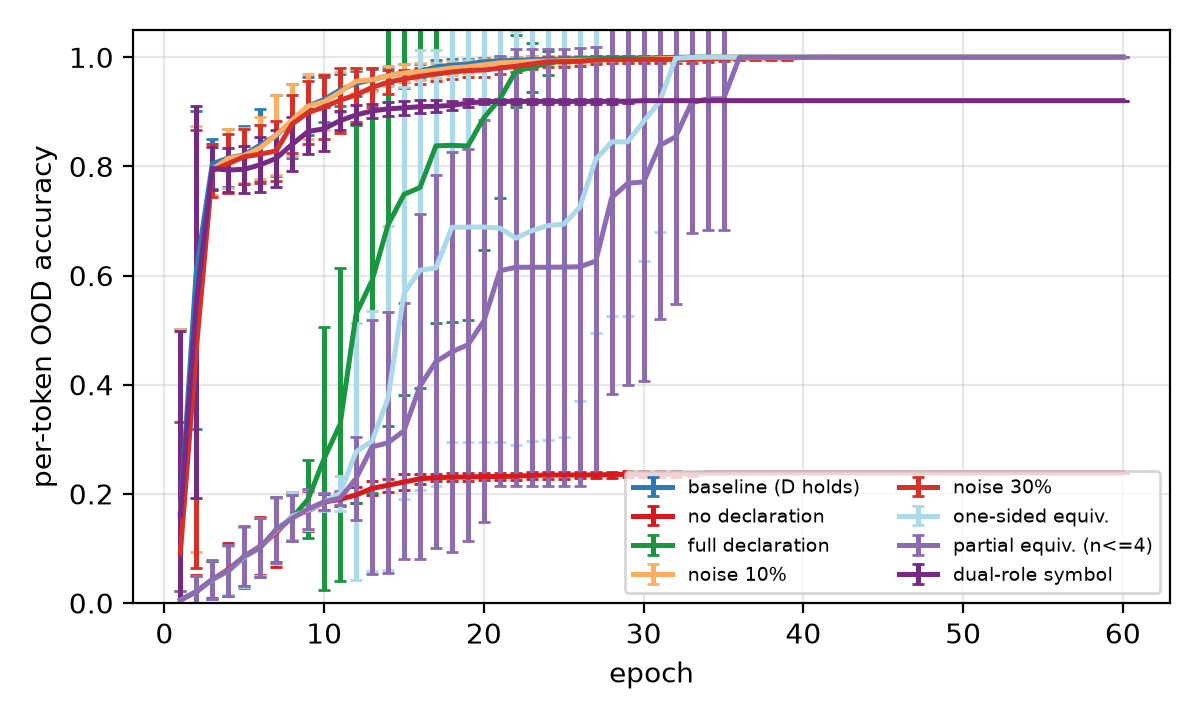
\includegraphics[width=0.95\textwidth]{fig1_curves.png}
\caption{Per-token OOD accuracy over epochs, by condition (mean
$\pm$ std over 3 seeds). The failing conditions (dual-role symbol,
no declaration) plateau below 1.0; noise slows recovery without
preventing it.}
\label{fig:curves}
\end{figure}

\begin{table}[h]
\centering
\small
\resizebox{\textwidth}{!}{%
\begin{tabular}{lccccc}
\toprule
Condition & $n$ & hit-one & per-token OOD & peak epoch & $p$ (vs.\ base) \\
\midrule
baseline ($D$ holds) & 10 & 10/10 & 1.000 & $22.7 \pm 5.1$ & --- \\
sample-count control (270) & 10 & 10/10 & 1.000 & $23.4 \pm 5.7$ & 0.72 \\
declaration complete (bridge) & 10 & 10/10 & 1.000 & $22.2 \pm 6.8$ & 0.86 \\
\emph{layering violated} (dual-role symbol) & 10 & \textbf{0/10} & $0.920$ & --- & --- \\
\emph{declaration absent} (no bridge) & 10 & \textbf{0/10} & $0.238$ & --- & --- \\
\emph{exclusion violated} (10\% noise) & 10 & 10/10 & 1.000 & $25.5 \pm 6.3$ & 0.29 \\
\emph{exclusion violated} (30\% noise) & 10 & 10/10 & 1.000 & $28.6 \pm 6.5$ & \textbf{0.04} \\
\emph{cancellation manipulation} (one-sided) & 10 & 10/10 & 1.000 & $25.7 \pm 7.4$ & 0.31 \\
\emph{cancellation manipulation} (partial coverage) & 10 & 10/10 & 1.000 & $27.9 \pm 6.2$ & 0.06 \\
\bottomrule
\end{tabular}
}
\caption{Decoupling ablation, dimension 64, 2 layers, 60 epochs, 10
seeds per condition. Hit-one: whether any epoch reaches per-token
OOD $=1.0$. Peak epoch: first epoch with per-token OOD $=1.0$ (mean
$\pm$ std); conditions that never hit 1.0 are marked ---. $p$:
two-sided Welch $t$-test of peak epoch against baseline
(Mann--Whitney agrees; appendix). The sample-count control adds 20
duplicated samples (270 total, matching the declaration
conditions) with no declaration content: no effect, ruling out
sample-count confounding.}
\label{tab:ablation}
\end{table}

\textbf{Layering violation (dual-role symbol).} We inject a symbol
that simultaneously plays two roles (operator and bracket). In all
ten seeds, sequence-level OOD is 0/32 while per-token OOD reaches
only $0.920$ --- roughly the fraction of the sequence that is not
the conflicted role. The model learns the statistics of both roles
but never resolves the mapping; the role confusion is not
repairable by more epochs (the curve is flat after the peak). This
is the strongest single effect in the ablation: layering is a
\emph{necessary} condition for OOD recovery.

\textbf{Missing declaration (no bridge).} Without the equivalence
declaration, per-token OOD plateaus at $0.238$ --- exactly the
shared-structure fraction --- and sequence-level OOD is 0/32 in all
seeds. The declaration is the only difference between this
condition and full recovery ($32/32$).

\textbf{Exclusion violations (noise injection).} Injecting
unrelated symbols into 10\%/30\% of each training sequence does
\emph{not} prevent recovery (hit-one 10/10 in both), but it slows
it: peak epoch $22.7 \pm 5.1$ (clean) $\to 25.5 \pm 6.3$ (10\%) $\to
28.6 \pm 6.5$ (30\%). The 30\% slowdown is significant against
baseline (Welch $t$-test $p = 0.038$, Mann--Whitney $p = 0.041$,
$n = 10$); the 10\% effect is in the same direction but not
significant ($p = 0.29$). The effect is in the direction predicted
by the condition (irrelevant material blurs declarations) and is
quantitative; we do not claim a mechanism beyond the observed
delay.

\textbf{Cancellation manipulations (weak or null effects).} We
tried two independent manipulations of the cancellation clause.
First, presenting equivalence samples with one side always on the
left: no significant effect (hit-one 10/10, peak epoch $25.7 \pm
7.4$, $p = 0.31$). Second, restricting the equivalence
declaration's coverage to $n \le 4$ while OOD requires the bridge
at $n \in \{10,11,12\}$: a borderline slowdown (peak epoch $27.9
\pm 6.2$, $p = 0.06$) --- the model largely generalizes the bridge
pattern from the declared range, with a possible small cost. Both
manipulations shift the peak epoch in the same direction
(slower), consistent with a weak real effect that the current
manipulations only partially instantiate; neither is fatal. We
report these results honestly: the samples' content is symmetric
in the first, and the declaration's \emph{pattern} is complete in
the second --- the model transfers the equivalence rule itself,
not its instances. The design of a true unpaired-declaration
manipulation --- a declaration whose counterpart is absent from
the signal --- remains open.

\textbf{Position-level decomposition.} The per-token label
decomposes into per-position labels: for each absolute position in
the probe sequence we record the epoch at which that position's OOD
accuracy first reaches 1.0 (or, if it never does, the epoch of its
maximal accuracy). The two failing conditions have sharply
different position patterns. In the missing-declaration condition,
only positions 0--1 (the judgment head and the outer bracket ---
the shared structure, present in every training sample) ever reach
1.0; every arithmetic-core position (the successor chains and the
operator) never does --- the per-token plateau of 0.238 is exactly
the shared-structure fraction. In the layering condition, the
dual-role symbol's bracket-role position (the outer bracket,
position 1) never reaches 1.0, and the interior positions it
encloses fail with it, while the operator position of the same
symbol recovers --- the role confusion is localized to the
conflicted role's positions rather than to the symbol as a whole. In the baseline, full-declaration,
exclusion, and one-sided conditions, every position reaches 1.0.
Position-level labels thus separate failure of the shared
structure from failure of the arithmetic core --- a distinction
that sequence-level accuracy (0/32 in both conditions) and even
overall per-token accuracy (0.238 versus 0.920) cannot make alone.
Figure~\ref{fig:positions} shows the per-position pattern.
Full per-position tables are in the appendix.

\begin{figure}[h]
\centering
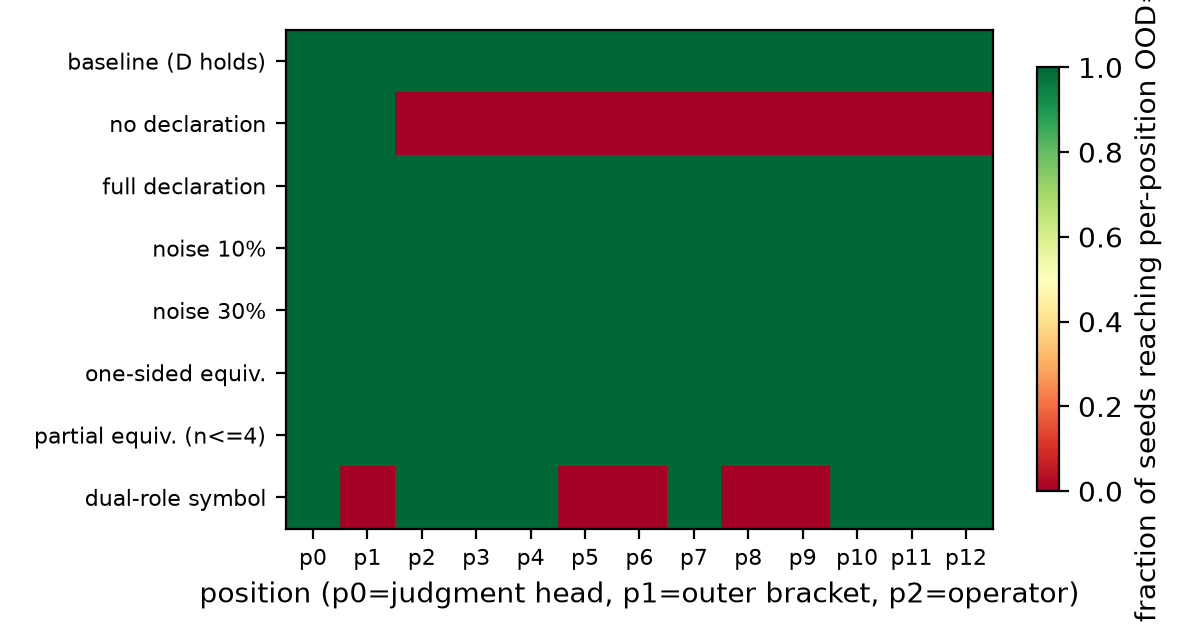
\includegraphics[width=0.95\textwidth]{fig2_positions.png}
\caption{Per-position hit-one (fraction of seeds whose per-position
OOD accuracy reaches 1.0). Position 0 = judgment head, 1 = outer
bracket, 2 = operator, 3+ = successor chains.}
\label{fig:positions}
\end{figure}

\textbf{Robustness across configurations.} Table~\ref{tab:robust}
shows baseline, full-declaration, and 30\%-noise conditions at
dimension 128 / 2 layers, 64 / 4 layers, and 128 / 4 layers (2
seeds each): hit-one is 2/2 in every configuration, and peak epochs
remain in the $18$--$29$ range. The two-pole pattern and the
ablation ordering are stable across model scale.

\begin{table}[h]
\centering
\small
\resizebox{\textwidth}{!}{%
\begin{tabular}{lcccc}
\toprule
Config & Condition & hit-one & per-token OOD (final) & peak epoch \\
\midrule
dim 128, 2 layers & baseline & 2/2 & 1.000 & $20.0 \pm 12.7$ \\
dim 128, 2 layers & full declaration & 2/2 & 1.000 & $19.0 \pm 8.5$ \\
dim 128, 2 layers & 30\% noise & 2/2 & 1.000 & $23.0 \pm 12.7$ \\
dim 64, 4 layers & baseline & 2/2 & 1.000 & $20.0 \pm 4.2$ \\
dim 64, 4 layers & full declaration & 2/2 & 1.000 & $26.0 \pm 14.1$ \\
dim 64, 4 layers & 30\% noise & 2/2 & 1.000 & $28.5 \pm 14.8$ \\
dim 128, 4 layers & baseline & 2/2 & 1.000 & $18.0 \pm 9.9$ \\
dim 128, 4 layers & full declaration & 2/2 & 1.000 & $28.5 \pm 26.2$ \\
dim 128, 4 layers & 30\% noise & 2/2 & 1.000 & $22.5 \pm 10.6$ \\
\bottomrule
\end{tabular}
}
\caption{Robustness across model configurations (2 seeds per cell).}
\label{tab:robust}
\end{table}

\section{Discussion}

\textbf{What the ablation shows.} The decoupling operator's clauses
are not symmetric in effect: layering and declaration are
\emph{necessary} (their violation blocks recovery), exclusion is
\emph{incremental} (its violation slows recovery monotonically),
and the one-sided-equivalence manipulation was a null result. The
necessary/ incremental distinction is itself a finding: it says
which design defects are fatal for OOD behavior and which are
costly-but-tolerable, and it gives a priority order for token-design
auditing.

\textbf{In-distribution versus OOD.} Training-set
per-token accuracy converges to 1.0 early in every condition
(appendix, Fig.~\ref{fig:idood}), so the OOD failure cannot be
attributed to incomplete training --- it is a
representation-bound transfer failure, not a learning failure.

\textbf{Anchor binding.} The position-level pattern of the
missing-declaration condition --- positions 0--1 (judgment head,
outer bracket) reach 1.0, all arithmetic-core positions do not ---
is direct evidence for anchor binding: the shared structure that
every training sample contains is the structure the model binds
and transfers, and the unshared arithmetic core is not. This is
the position-level form of the anchor-binding regularity observed
in the program's earlier experiments (E11), and it explains why
the per-token plateau is exactly the shared-structure fraction.

\textbf{Delayed OOD recovery.} In every condition that
recovers, per-token OOD reaches 1.0 only in the second half of
training (peak epochs 14--41 of 60). The OOD curve therefore has
the delayed-generalization shape documented in the grokking
literature \citep{power2022grokking}, with an important
difference: the delay here is \emph{representation-bound} --- the
same training schedule recovers or fails depending only on the
token design, not on dataset size or weight decay. The peak-epoch
label makes this comparison quantitative.

\textbf{Per-token OOD as a diagnostic.} Sequence-level accuracy
collapses to 0/32 in both the layering and the no-declaration
conditions, but the per-token view separates them: $0.920$ (one
role unresolved) versus $0.238$ (all arithmetic content
unresolved). The peak-epoch label adds the time dimension: the
exclusion effect is invisible at the endpoint (1.000 in both cases)
and visible only in the curve. We recommend per-token OOD curves
and peak-epoch labels as standard diagnostics for symbolic-training
experiments.

\textbf{Relation to prior work.} The two-pole pattern is the
representation-bound side of the systematic-generalization and
length-extrapolation literatures
\citep{lake2018generalization, keysers2020measuring,
hupkes2020compositionality, bahdanau2019systematic, anil2022exploring,
jelassi2023length, raffel2020exploring, zhou2021open,
qiu2020pretrained}: those works vary data and architecture; we vary
the token design while holding data distribution and architecture
fixed. The conditions give a vocabulary for \emph{why} a given
design fails, and the ablation gives per-clause evidence.

\section{Honest boundary}

First, the four conditions are generalizations from one research
program's process --- one token system, one experiment family, one
collaboration; they are not claimed to hold for all possible token
systems. Second, the empirical-to-framework correspondence is
observational: the experiments exhibit the conditions, they do not
prove them. Third, the Lean formalization verifies the verdict
structure, not the experimental claims. Fourth, the authorship and
provenance situation is stated in the AI assistance statement above
and is not repeated here. Fifth, the conditions exclude the
informal channels by which a representation can also carry
influence --- emotion, linguistic bias, suggestion; these are not
legal presentations and not norm symbols under the present
conditions, and the framework records only that they exist and are
unjudged here. Sixth, legality is the minimum standard, not
the full standard. A presentation can be fully legal and still
poor: the parenthesis-free notation is unambiguous --- the strong
form of legality --- yet is read with difficulty, and a token
system can satisfy every resolvability condition while imposing
high cognitive load, low naturalness, or poor maintainability.
Reader-friendliness --- readability, cognitive load, naturalness,
maintainability --- is a real dimension of presentation quality,
and it is deliberately outside the present conditions: the
conditions judge legality, and take no position on the further
dimension, which belongs to cognitive and human-factors research.
Seventh, the claims are kept minimal by discipline:
every claim is restricted to what the experiments show; the
philosophical lineages and the continuations are positioned as
context, not as result. Eighth, what remains open: (1) whether the
decoupling clauses suffice for other token systems (natural-language
corpora, visual symbols); (2) a norm checker that \emph{computes}
whether a given symbol system is norm; (3) a grammar-based detector
of undeclared coincidences; (4) whether the two-pole comparison can
be applied before training as a filter on proposed token designs;
and (5) a true unpaired-declaration manipulation for the
cancellation clause. These continuations are stated so that each
condition's boundary is visible: each rule stops where the next
researcher can begin.

\section{Related work}

\paragraph{Algorithmic generalization.}
Delayed generalization \citep{power2022grokking}, the Chomsky
hierarchy \citep{deletang2022chomsky}, compositional
generalization \citep{lake2018generalization, keysers2020measuring,
hupkes2020compositionality, bahdanau2019systematic}, length
extrapolation \citep{anil2022exploring, jelassi2023length,
raffel2020exploring, press2021alibi, su2021roformer}, and neural
mathematics \citep{saxton2019analysing, lample2020deep,
hendrycks2021measuring, razeghi2022impact} study the same
generalization question from the data and architecture side; we
hold both fixed and vary the token design.

\paragraph{Representation and symbols.}
The symbol-meaning separation has classical sources in
semiotics and philosophy of language \citep{saussure1916course,
peirce1931collected, frege1892sense, quine1960word,
wittgenstein1953investigations, chomsky1957syntax}; the training
side is representation-bound statistics \citep{lecun2015deep}.

\paragraph{Intuition and its conditions.}
The two-pole precision condition is the operational form of the
conditions for intuitive expertise \citep{kahneman2011thinking,
kahneman2009conditions, gigerenzer2011heuristic, evans2013dual,
dehaene1997number}.

\paragraph{Formalization.}
The verdicts are formalized in Lean 4 / mathlib
\citep{lean4, mathlib2020, mathlib2026, demoura2015lean,
avigad2018mechanization, buzzard2022rise, hales2017kepler}.

\section{Conclusion}

The pattern is reproduced, the conditions are stated and
formalized, and the ablation gives per-clause evidence for which
design defects are fatal and which are costly-but-tolerable. The
two-pole pattern is stable across model scale; the per-token OOD
curve is a diagnostic that separates failure modes that
sequence-level accuracy conflates. Within the boundary of
Section~8, the four conditions are this program's answer to the
question its failures asked: what does it take, in this program's
setting, for a symbolic training signal to generalize
out-of-distribution?

\bibliographystyle{iclr2026_conference}
\bibliography{refs}


\appendix
\section{In-distribution versus OOD curves}
\label{app:idood}

\begin{figure}[h]
\centering
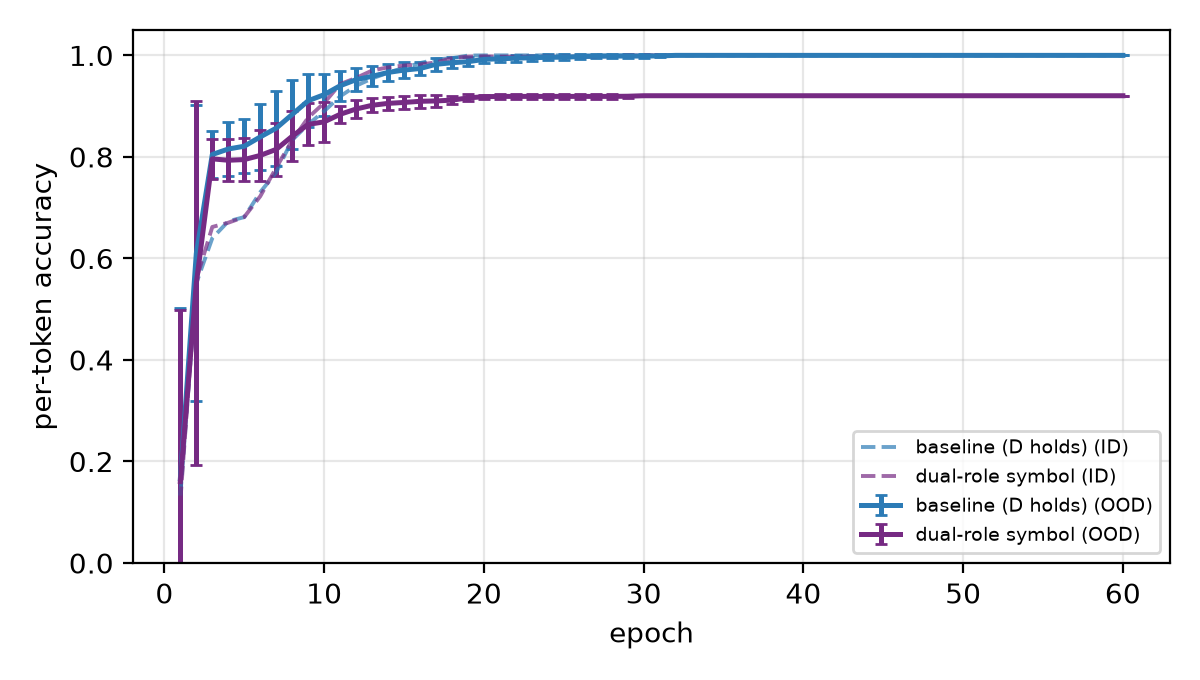
\includegraphics[width=0.8\textwidth]{fig4_id_ood.png}
\caption{Per-token accuracy on the training set (ID, dashed) and on
OOD probes (solid), for baseline and the dual-role condition. ID
converges to 1.0 in both; OOD separates them.}
\label{fig:idood}
\end{figure}

\section{Full experimental configuration}
\label{app:config}

\textbf{Training.} TokenTransformer (causal=False), dimension 64
(robustness: 128), 2 layers (robustness: 4), 60 epochs, Adam
$\mathrm{lr}=10^{-3}$, batch size 512, position cross-entropy
(rewarding correct positions) plus validity cross-entropy
(correct/wrong distinction), weighting $w_\mathrm{valid}=0.5$.
Seeds 0,1,2 (robustness: 0,1). Hardware: single GPU (CUDA 13.0,
torch 2.11.0); one run of 60 epochs takes approximately 2.4
seconds.

\textbf{Data.} 250 successor-notation arithmetic samples: addition
($m,n \le 9$) and multiplication ($m,n \le 4$) facts, each with a
true case (chain of length $k$) and a false case (chain of length
$k+1$), assembled through the five-layer token system's API.
OOD probes: 32 samples with $m,n \in \{10,11,12\}$ (length
extrapolation beyond the training range) for each notation.

\textbf{Ablation manipulations.}
\begin{itemize}
\item \emph{layering violation}: a symbol injected with two roles
(operator and bracket); samples assemble the operator role and
wrap the expression with the bracket role of the same symbol.
\item \emph{declaration absent}: equivalence samples (bridge)
excluded from training; OOD probed in the unbridged notation.
\item \emph{exclusion violation}: a defined-but-unreferenced
symbol inserted into 10\%/30\% of each training sequence at random
positions.
\item \emph{cancellation manipulation}: equivalence samples
presented with one side always on the left.
\end{itemize}

\section{Position-level patterns}
\label{app:pos}

Table~\ref{tab:pos} shows, for each condition of the main
configuration, the positions that reach per-position OOD accuracy
1.0 (hit-one per position, 3 seeds consistent): position 0 is the
judgment head (\texttt{is\_true}), position 1 the outer bracket,
and positions 2+ the operator and successor chains. Full per-position
curves are in the artifact (\texttt{results/ablation\_pos\_curve.tsv},
per-position summary \texttt{ablation\_pos\_summary.tsv}).

\begin{table}[h]
\centering
\small
\resizebox{\textwidth}{!}{%
\begin{tabular}{lccccccccccccc}
\toprule
Condition & p0 & p1 & p2 & p3 & p4 & p5 & p6 & p7 & p8 & p9 & p10 & p11 & p12 \\
\midrule
baseline & 1 & 1 & 1 & 1 & 1 & 1 & 1 & 1 & 1 & 1 & 1 & 1 & 1 \\
no\_decl & 1 & 1 & 0 & 0 & 0 & 0 & 0 & 0 & 0 & 0 & 0 & 0 & 0 \\
decl\_full & 1 & 1 & 1 & 1 & 1 & 1 & 1 & 1 & 1 & 1 & 1 & 1 & 1 \\
excl\_pollute30 & 1 & 1 & 1 & 1 & 1 & 1 & 1 & 1 & 1 & 1 & 1 & 1 & 1 \\
canc\_1side & 1 & 1 & 1 & 1 & 1 & 1 & 1 & 1 & 1 & 1 & 1 & 1 & 1 \\
layer\_dual & 1 & 0 & 1 & 1 & 1 & 0 & 0 & 1 & 0 & 0 & 1 & 1 & 1 \\
\bottomrule
\end{tabular}}
\caption{Per-position hit-one (whether the position's OOD accuracy
ever reaches 1.0; 1 = yes, 0 = no, consistent across 3 seeds).
Position 0 = judgment head, 1 = outer bracket, 2 = operator,
3+ = successor chains.}
\label{tab:pos}
\end{table}

\section{Statistical tests and per-seed detail}
\label{app:seeds}

Per-seed labels for all 108 runs are in the artifact
(\texttt{results/ablation\_summary.tsv}); full per-epoch and
per-position curves in \texttt{ablation\_curve.tsv} and
\texttt{ablation\_pos\_curve.tsv}. Table~\ref{tab:stats} reports
the two-sided Welch $t$-test and Mann--Whitney $U$ of peak epoch
against baseline ($n = 10$ per condition).

\begin{table}[h]
\centering
\small
\begin{tabular}{lcccc}
\toprule
Condition vs.\ baseline & $\Delta$ peak epoch & Welch $t$ & $p$ ($t$) & $p$ (M--W) \\
\midrule
sample-count control (270) & $+0.7$ & 0.36 & 0.72 & 0.78 \\
declaration complete & $-0.5$ & 0.19 & 0.86 & 0.73 \\
exclusion 10\% noise & $+2.8$ & $-1.09$ & 0.29 & 0.36 \\
exclusion 30\% noise & $+5.9$ & $-2.25$ & \textbf{0.038} & \textbf{0.041} \\
cancellation one-sided & $+3.0$ & $-1.06$ & 0.31 & 0.31 \\
cancellation partial coverage & $+5.2$ & $-2.04$ & 0.057 & 0.059 \\
\bottomrule
\end{tabular}
\caption{Peak-epoch comparisons against baseline ($n = 10$ per
condition). Two-sided tests; Mann--Whitney is the non-parametric
counterpart.}
\label{tab:stats}
\end{table}

\end{document}
